\section{绘画}\label{sec:painting}
在当今数字化时代,GPT 不仅在文本处理领域大放异彩,在辅助绘画方面也展现出强大的功能。它能够帮助创作者实现多种复杂的图像操作,极大地拓展了绘画创作的边界。
利用 GPT 的图像超分辨率技术,可以将低分辨率(1k)的图像无损地提升至高分辨率(4k)。这一过程通过深度学习算法对图像中的细节进行智能补充和重建,使得原本模糊的图像变得更加清晰锐利,满足对高清图像的需求,比如在印刷、大型展示等场景下的应用。GPT 可以精准识别图像主体与背景,通过算法自动去除背景,留下干净的主体图像。这对于需要将主体单独提取出来用于合成、设计等工作非常方便,大大节省了手动抠图的时间和精力。只需简单的指令,GPT 就能将图像的颜色进行反转,即黑变白、白变黑,其他颜色也相应反转。这种操作在一些创意设计、艺术创作中能带来独特的视觉效果,也有助于图像分析等工作。
当图像存在噪点影响视觉效果时,GPT 能够运用其去噪算法,智能识别并去除噪点,使图像恢复清晰、平滑,提升图像质量。用户可以向 GPT 输入想要替换的背景描述,如 “将当前图像背景替换为蓝天白云的草原场景”,GPT 会根据描述生成新的背景,并与原图像主体完美融合,创造出全新的画面效果。同样,若要替换图像中的人物,只需提供新人物的特征描述,如 “将画面中的人物换成一位穿着古装的女子”,GPT 就能完成人物替换,同时保证整体画面的协调性和逻辑性。无论是想要一张科幻风格的城市夜景图,还是温馨的家庭生活场景图,只要给出详细的需求,如 “生成一张未来城市中飞行汽车穿梭的图片,城市中有绚丽的霓虹灯和高楼大厦”,GPT 就能按照要求生成满足特定需求的高质量图片。GPT 可以根据文本描述生成各种想象中的场景。比如,当输入 “生成一个古代仙侠世界中的神秘山谷,山谷中有清澈的溪流、奇形怪状的石头和盛开的花朵”,它能迅速构建出相应的场景画面,为绘画创作者提供丰富的灵感和基础素材,大大加快创作进程。用户可以指定将一种图像风格迁移到另一种图像上。例如,将梵高的油画风格应用到一张普通的风景照片上,GPT 会分析梵高油画的笔触、色彩特点等,然后将这些风格元素融入到目标图像中,使其具有梵高油画的独特艺术风格。



\subsubsection{图像风格转移}\label{ux6848ux4f8b3ux5c06ux62cdux6444ux7684ux7167ux7247ux4feeux6539ux4e3aux52a8ux6f2bux98ceux683c}}

\textbf{操作流程:}

\begin{enumerate}
  \def\labelenumi{\arabic{enumi}.}

  \item
        访问\href{https://huggingface.co/spaces/timbrooks/instruct-pix2pix}{InstructPix2Pix
          - a Hugging Face Space by
          timbrooks},这是一个根据提示词将图片修改变换的模型
  \item
        填写参数,下图中的红框是上传你要修改的图片;蓝框则是你的提示词(推荐使用英语尽可能简短地描述你的需求);绿框则是一些参数的调整,Text
        CFG是提示词的权重,Image
        CFG是图片的权重,读者可以通过调整这两个主要参数来实现目标,但同时要注意两者之间的平衡,否则会导致图像失真或者生成完全不符合要求的图片。
\end{enumerate}

\centering
\begin{figure}[H] %H为当前位置,!htb为忽略美学标准,htbp为浮动图形
  \centering %图片居中
  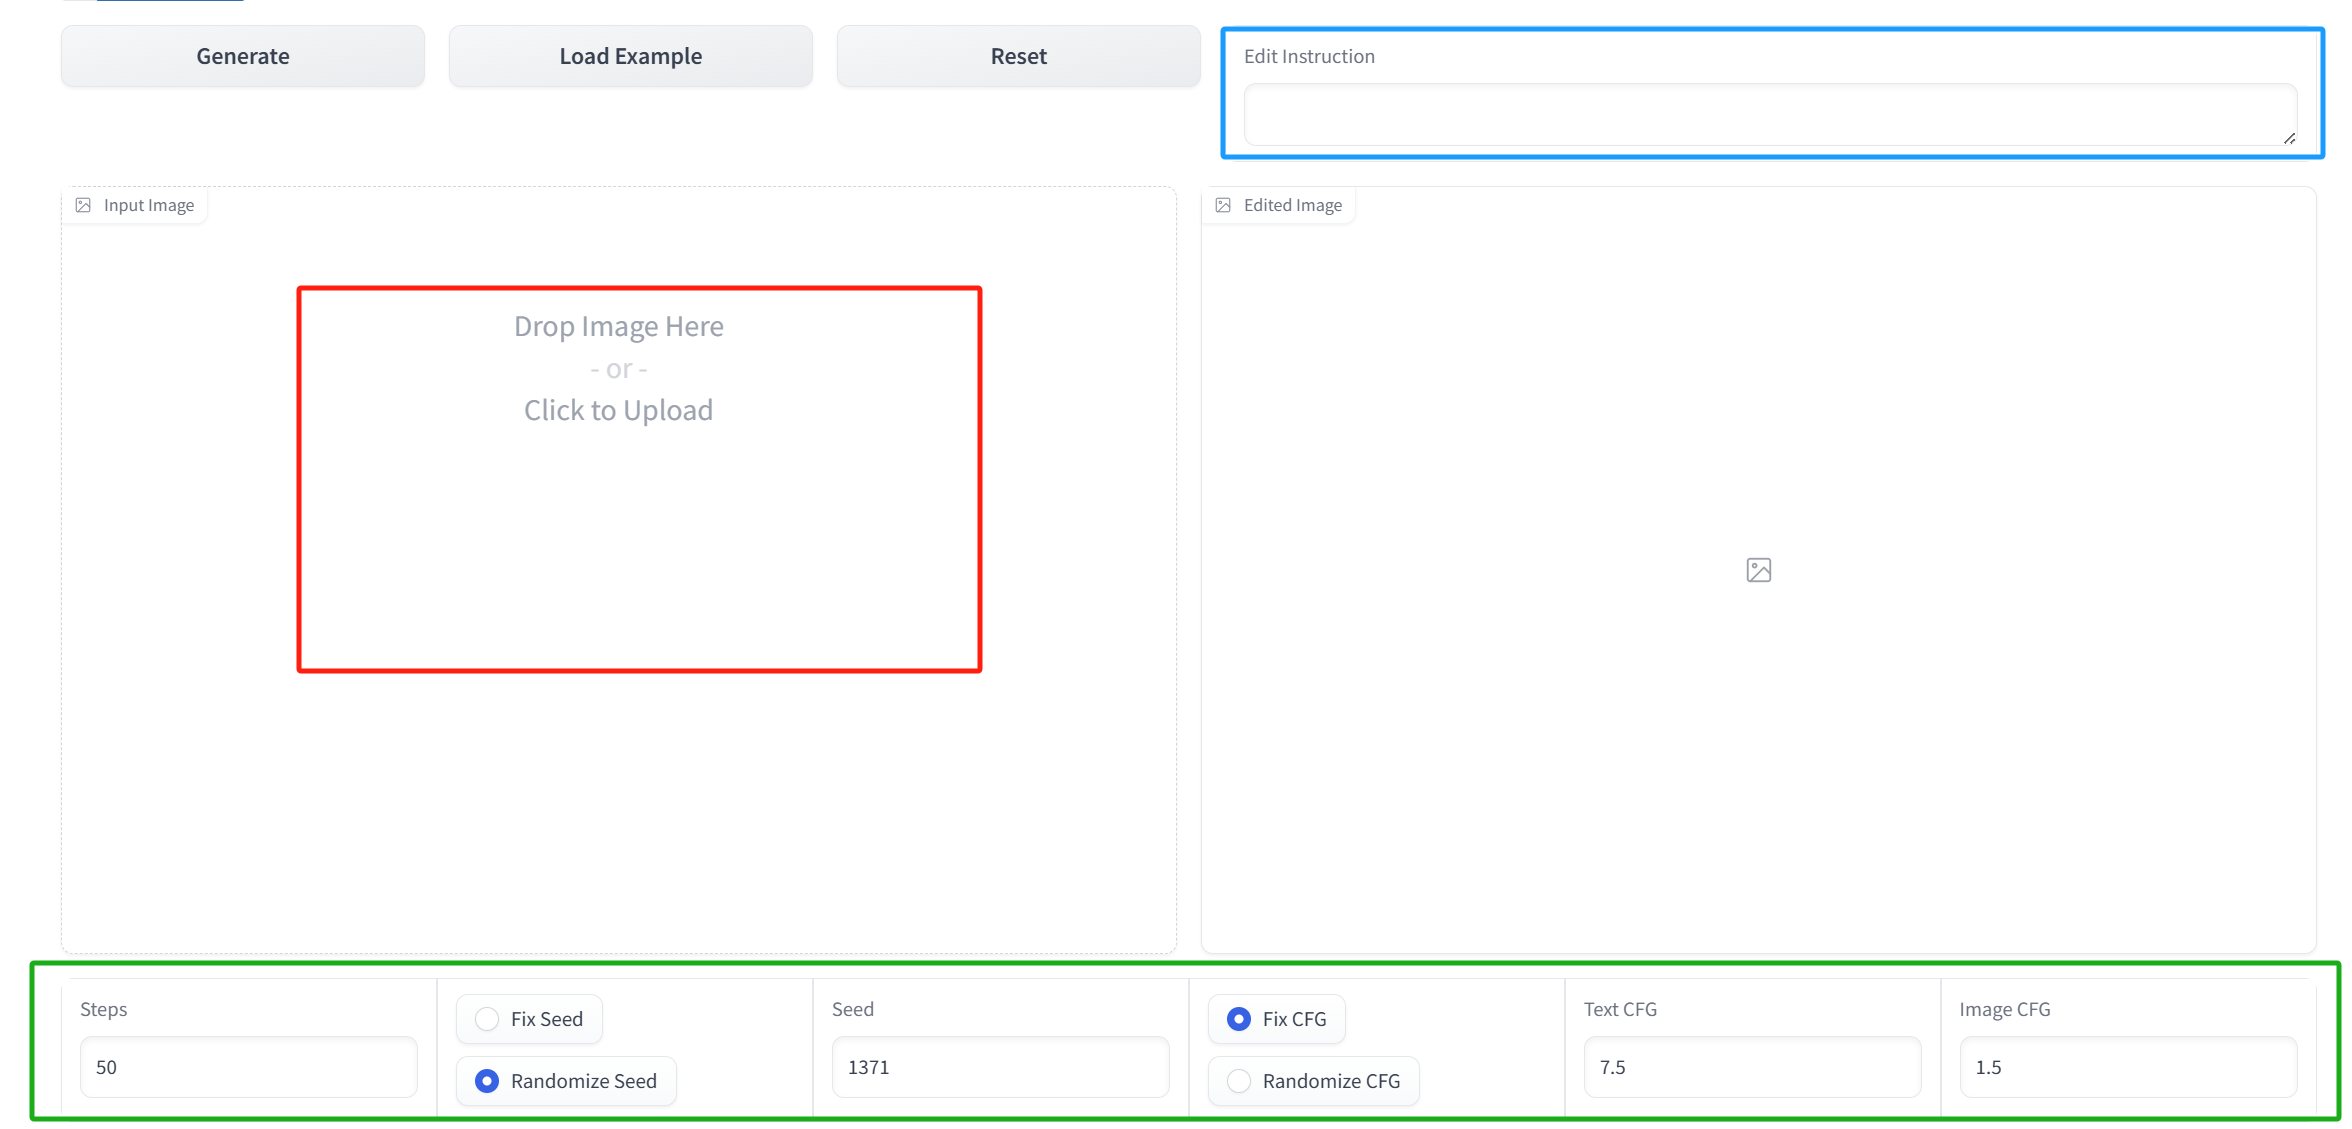
\includegraphics[width=0.7\textwidth]{assets/figures/image-20250211145347208.png} %插入图片,[]中设置图片大小,{}中是图片文件名
  \caption{参数调整} %最终文档中希望显示的图片标题
  \label{Fig.main1} %用于文内引用的标签
\end{figure}%结束环境

例如:将云南师范大学的照片转化为动漫风格,我的参数和提示词如下图
\centering
\begin{figure}[H] %H为当前位置,!htb为忽略美学标准,htbp为浮动图形
  \centering %图片居中
  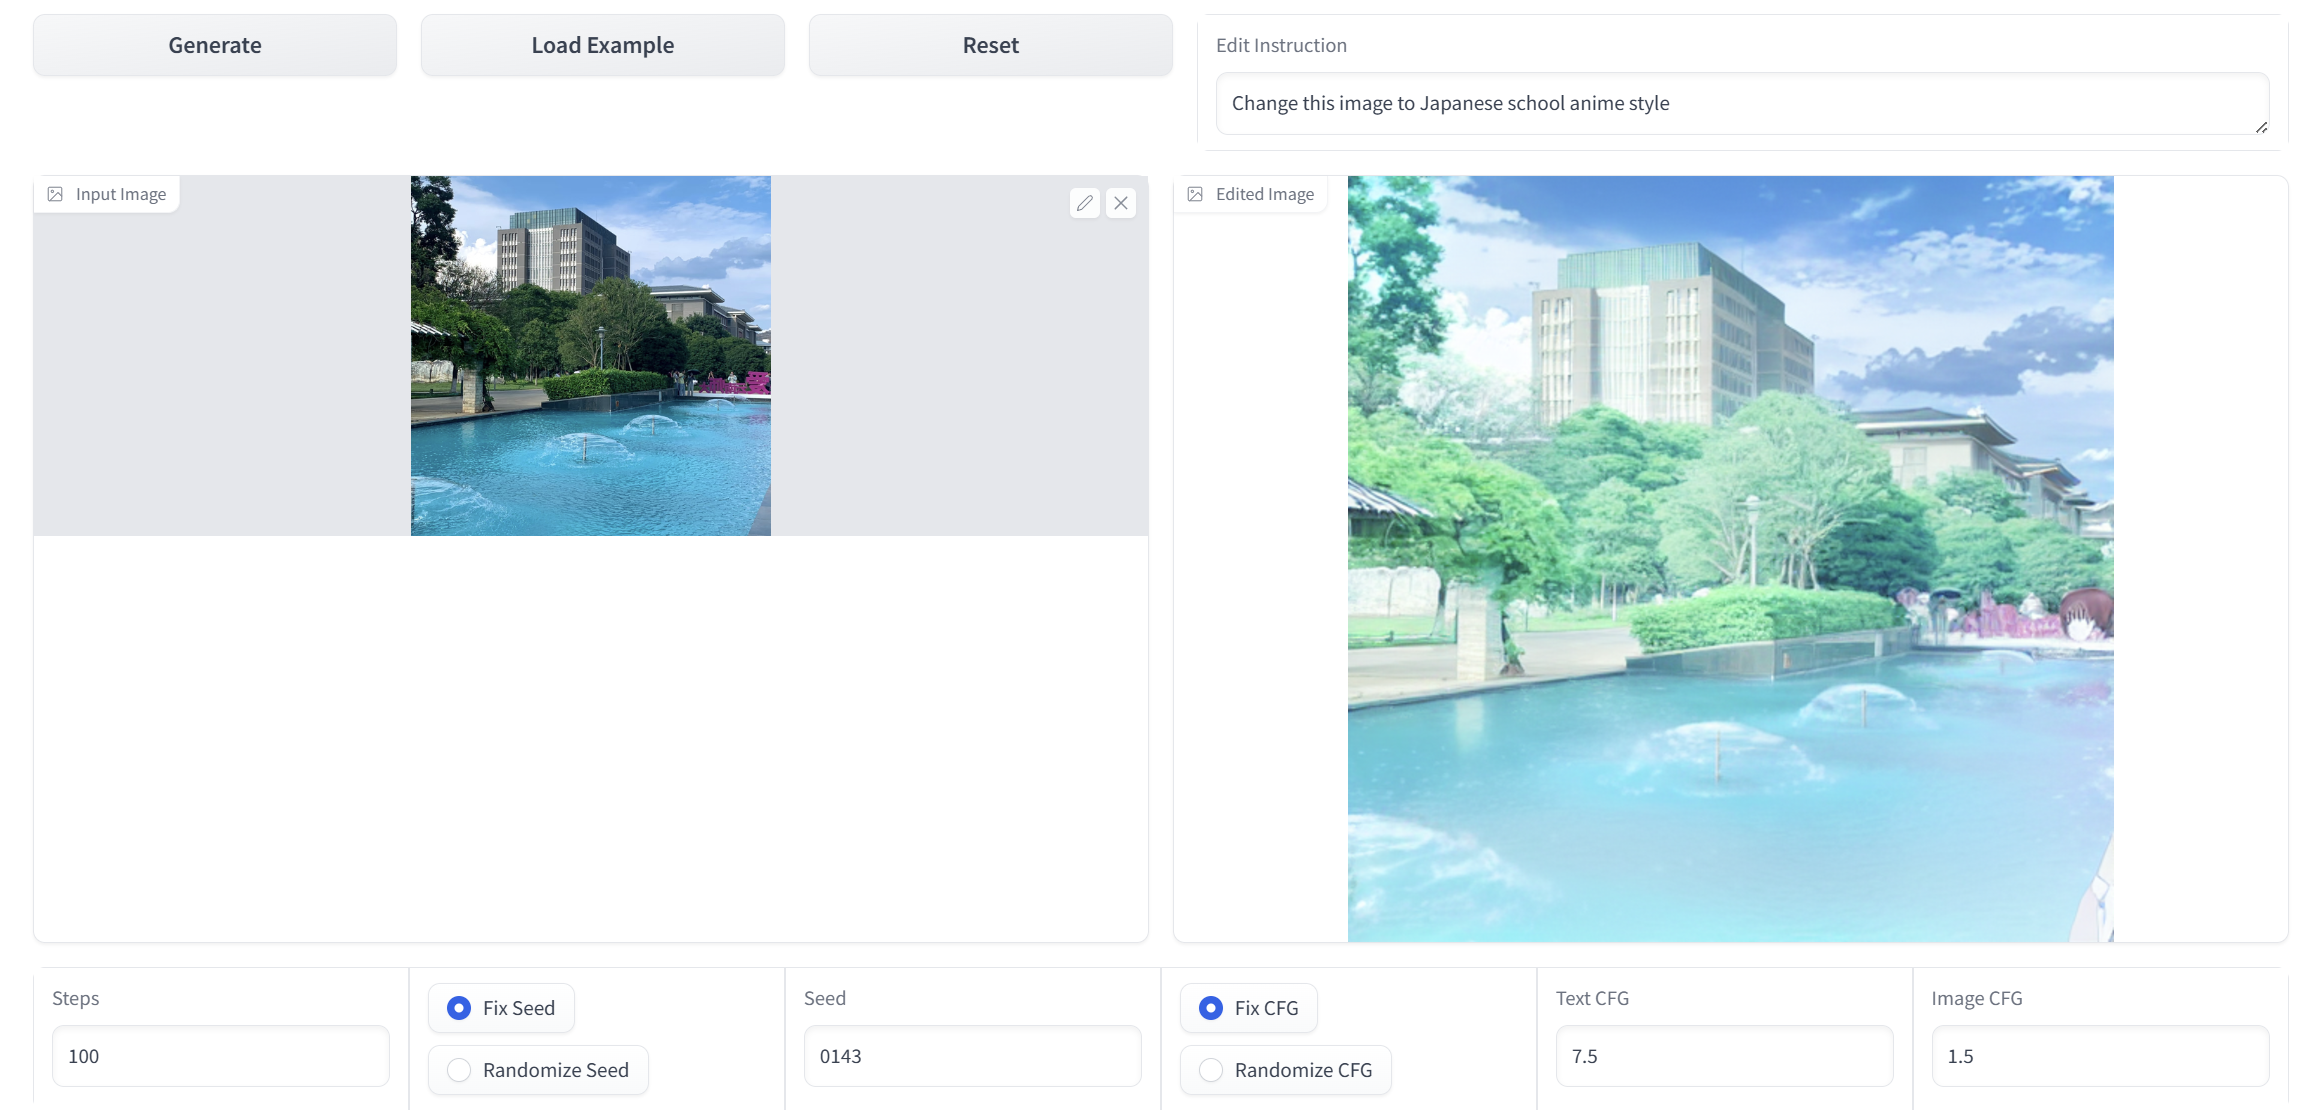
\includegraphics[width=0.7\textwidth]{assets/figures/9c6c2ff0409374eed093b8ec3447507.png} %插入图片,[]中设置图片大小,{}中是图片文件名
  \caption{渲染过程} %最终文档中希望显示的图片标题
  \label{Fig.main1} %用于文内引用的标签
\end{figure}%结束环境

\centering
\begin{figure}[H] %H为当前位置,!htb为忽略美学标准,htbp为浮动图形
  \centering %图片居中
  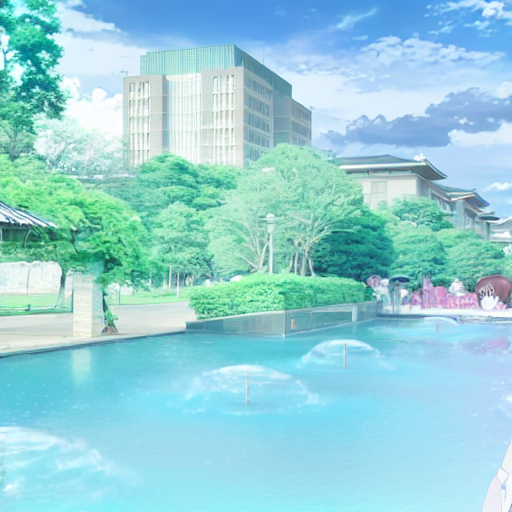
\includegraphics[width=0.7\textwidth]{assets/figures/change.png} %插入图片,[]中设置图片大小,{}中是图片文件名
  \caption{渲染效果图} %最终文档中希望显示的图片标题
  \label{Fig.main1} %用于文内引用的标签
\end{figure}%结束环境

可以看到还是改变了一点风格,读者可以继续尝试不断修改参数来达到预期的目标


% 以liblib为例(网址:https://www.liblib.art)

% 1、文生图:
% 选择模型:基础算法_F.1.safetensors
% 提示词:This is a photograph of a detailed, stylized doll in a fantastical setting. The doll is a small, cute, androgynous figure with light blue hair styled in a high ponytail, large expressive blue eyes, and a serious expression. The doll wears a traditional Chinese white robe with a blue sash, featuring intricate blue and gold embroidery on the sleeves and hem. The robe is slightly transparent, revealing a darker blue undergarment. The doll stands on a textured, rocky surface, with water-like elements splashing around it, creating a mystical, otherworldly atmosphere. The background is a surreal, ethereal landscape of blue and white, with what appears to be a temple or ancient building in the distance. The lighting is soft and ethereal, enhancing the mystical feel of the scene. The doll's pose is slightly forward, with hands outstretched, as if beckoning or offering something. The overall composition and color palette evoke a sense of ancient Chinese mythology or fantasy.
% 效果:


% 图生图 风格迁移
